\label{sez:interfaccia}



\begin{figure}[]
	\centering
	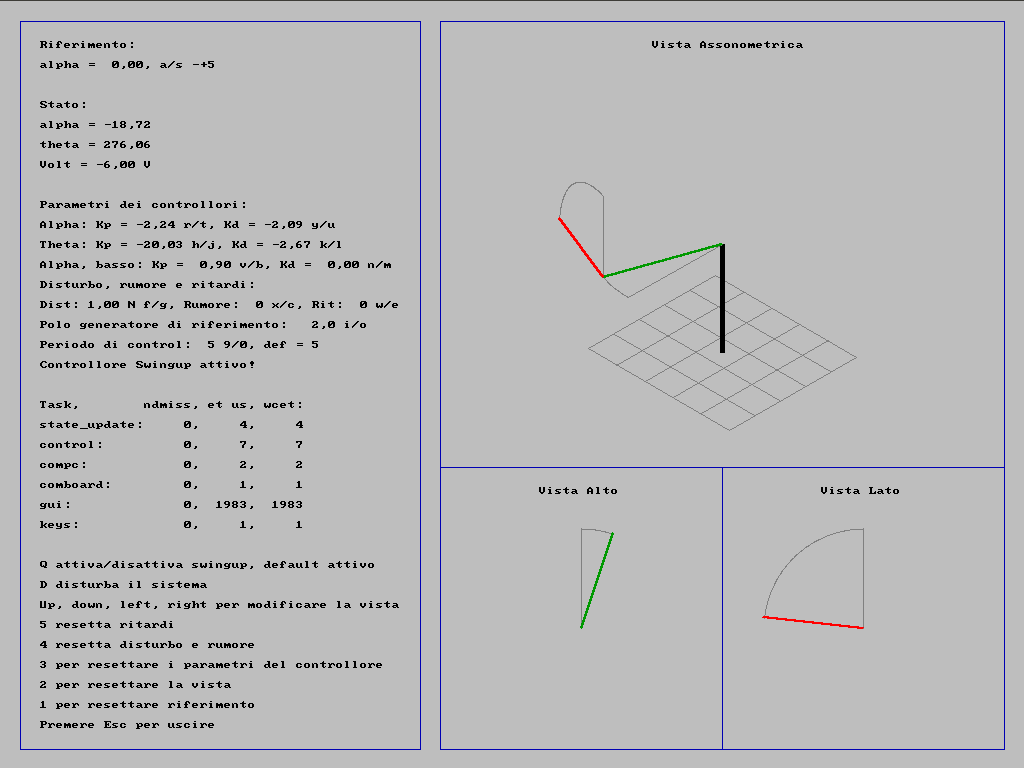
\includegraphics[height=.4\textheight]{interfaccia_in_esecuzione.png}
	\caption{Interfaccia durante l'esecuzione}
	\label{fig:interfaccia_in_esecuzione}
\end{figure}

L'interfaccia \`e divisa in due zone principali: quella di comunicazione con l'utente e le tre viste del pendolo.

Per quanto riguarda la zona di comunicazione questa \`e popolata dalle variabili di interesse e i modi con i quali modificarle. Si \`e quindi riportato a schermo:
\begin{itemize}
	\item il riferimento su $\alpha$
	\item  il vettore di stato $\left[ \alpha \ \theta \ volt\right]^T$
	\item i parametri di controllo	
	\item disturbo, rumore e ritardo	
	\item polo della funzione di trasferimento che genera il riferimento su $\alpha$
	\item periodo del task di controllo
	\item per ciascun task il numero di deadline miss, il tempo di esecuzione in $\si{\micro \second}$ e il worst-case execution time in $\si{\micro \second}$
	\item varie istruzioni su come resettare e come uscire dal programma
\end{itemize}

\begin{figure}[]
	\centering
	\def\svgwidth{0.7\linewidth}
	\input{draw2_withaxis.pdf_tex}
	%	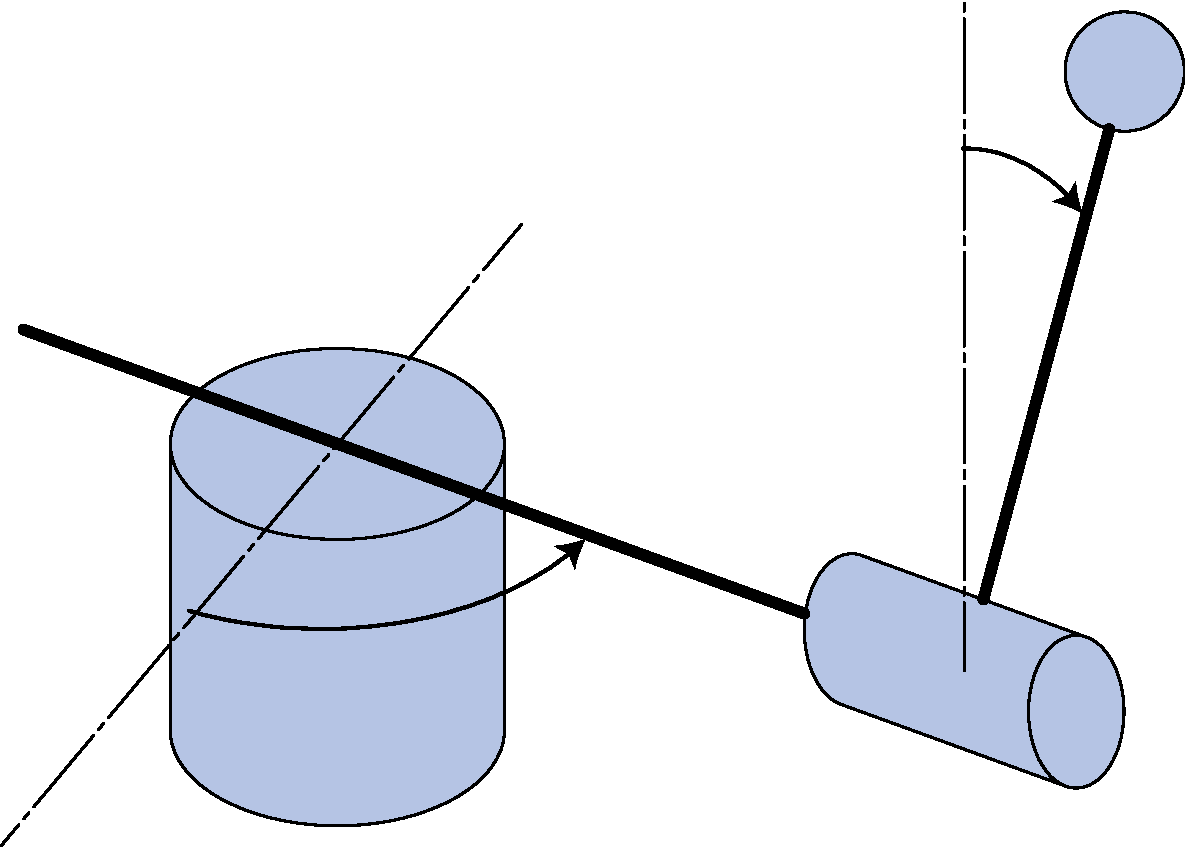
\includegraphics[width=.7\linewidth]{schema_2.pdf}
	\caption{Schema del Pendolo}
	\label{fig:pendolo_schema}
\end{figure}

Per quanto riguarda le viste, ne sono riportate tre. La scelta di rappresentare il pendolo attraverso tre viste \`e funzionale a valutare l'efficacia dell'azione di controllo sui singoli angoli.
Tramite la vista dall'alto viene messa in evidenza la posizione corrente del primo link, in verde, e la posizione desiderata, in grigio. Lo stesso viene fatto per il secondo link, in rosso, per mezzo della vista laterale.

Attraverso la terza vista, ovvero quella assonometrica, si rappresenta la struttura complessiva del pendolo che rende pi\`u intuitiva la comprensione dello stato attuale del sistema. Al fine di facilitare l'osservazione del pendolo durante il suo moto, \`e stato deciso di rendere tale vista interattiva, consentendo all'utente di spostare il punto di vista rispetto al quale osserva il sistema.

 Facendo riferimento alla figura~\ref{fig:pendolo_schema}, i punti di interesse per disegnare il pendolo sono $O$, $A$ e $P$, rispettivamente i punti intorno ai quali ruotano il primo link, il secondo link e l'estremit\`a di quest'ultimo. I sistemi di riferimento intermedi, utilizzati per la parametrizzazione del problema, sono riportati in figura~\ref{fig:pendolo_schema}. Per agevolare lo sviluppo delle relazioni che legano un qualsiasi punto dello spazio fisico ad un punto nel piano immagine dell'interfaccia \`e risultato utile strutturare il problema in coordinate omogenee in quanto permettono di rappresentare le rototraslazioni come trasformazioni lineari. Queste vengono rappresentate da un'unica matrice $^i T_{ij}$ composta da $R_i(\varphi)$,  generica rotazione intorno all'asse $i$ di un angolo $\varphi$, e da $^i d_{ij}$ vettore congiungente le origini dei sistemi di riferimento $i$ e $j$ scritto in coordinate $i$:
 \begin{equation}
	 ^i\! T_{ij}(\varphi) = \left[ \begin{array}{ccc|c}
	 & & & \\
	 & R_z(\alpha) & & ^i d_{ij} \\
	 & & & \\
	 \hline
	 0 & 0 & 0 & 1
	 \end{array} \right]
 \end{equation}
Per il generico vettore posizione scritto in coordinate omogenee vale la seguente relazione di cambio sistema di riferimento: $^ip = T_{ij}\ ^j p$. Nel caso in esame sono state utilizzate le seguenti matrici:
\begin{equation}
	^0\! T_{01}(\alpha) = \left[ \begin{array}{ccc|c}
	& & & l_1 \\
	& R_z(\alpha) & & 0 \\
	& & & 0 \\
	\hline
	0 & 0 & 0 & 1
	\end{array} \right]
	\quad 
	^1 T_{12}(\vartheta) =
	\left[  \begin{array}{ccc|c}
	& & & 0 \\
	& R_x(- \vartheta) & & 0 \\
	& & & 0 \\
	\hline
	0 & 0 & 0 & 1
	\end{array}
	\right]
\label{eq:cambio_coordinate}
\end{equation}
Con queste sono state quindi ricavate le coordinate in sistema di riferimento $0$ dei punti di interesse:
\begin{equation}
	\begin{aligned}
	^0\!\mathrm{OA} = &\left[ \begin{array}{c} l_1 \cos\alpha \\ l_1 \sin \alpha \\ 0 \end{array}\right] \\
	^0\!\mathrm{OP} = &\left[ \begin{array}{c} l_1 \cos \alpha - l_2 \sin \alpha \sin \vartheta\\ l_1 \sin \alpha + l_2 \cos \alpha \sin \vartheta\\ l_2 \cos \vartheta \end{array}\right]
	\end{aligned}
\end{equation}
Per poter rappresentare su schermo il pendolo \`e necessario infine proiettare le coordinate spaziali dei punti ottenute in uno spazio bidimensionale. A tale scopo viene utilizzata la seguente relazione, in cui si indicano con $s$ gli assi assonometrici, con $\rho$ l'angolo di longitudine e con $\lambda$ quello di latitudine:
\begin{equation}
	R_{s0} = R_z (\rho)  R_y (-\lambda)  \begin{bmatrix}
	0 & 0 & -1\\
	1 & 0 & 0\\
	0 & -1 & 0
	\end{bmatrix}
\label{eq:proiezione}
\end{equation}
In questa \`e stato incluso il cambio orientazione necessario per passare al sistema di coordinate di Allegro.
Il generico punto $^0\!\left[ x \ y \ z \right]^t $ risulta avere componenti:
\begin{equation}
	x_{s} = x\sin\rho + y\cos\rho, \quad y_{s} = x \cos \rho \sin \lambda + y \sin \lambda \sin \rho - z \cos \lambda
\end{equation}